%%% Kapitola 2: Specifikace požadavků

\chapter{Specifikace požadavků}
\label{chap:specifikace}

Tato kapitola definuje požadavky na systém -- uživatelskou roli, uživatelské
příběhy (user stories), případy užití (use cases) a~z~nich odvozené funkční
a~nefunkční požadavky.

%%% -----------------------------------------------------------------------
\section{Uživatelské role}
\label{sec:role}

Systém definujeme pro jedinou uživatelskou roli -- \textbf{uživatele Bitcoinové
peněženky}. Tento uživatel vlastní hardwarovou peněženku Trezor a~chce prostřednictvím
mobilní aplikace na platformě Android spravovat své Bitcoinové prostředky. Uživatel
požaduje pokročilé funkce, které mu běžné mobilní peněženky neposkytují:

\begin{itemize}
  \item \textbf{Multisignature transakce} -- možnost vytvářet a~podepisovat transakce
        vyžadující souhlas více klíčů (schéma M-of-N).
  \item \textbf{Coin control} -- manuální výběr konkrétních nepoužitých výstupů
        (UTXO) při tvorbě transakcí.
  \item \textbf{Integrace s~hardwarovou peněženkou} -- veškeré podepisování transakcí
        probíhá výhradně na zařízení Trezor; server nikdy nedisponuje privátními klíči.
\end{itemize}

Předpokládáme, že uživatel má základní znalost fungování Bitcoinu a~je obeznámen
s~konceptem hardwarových peněženek. Systém nepočítá s~rolí administrátora ani
s~víceuživatelským režimem -- každá instance backendu obsluhuje jednoho uživatele
s~jeho účty.

%%% -----------------------------------------------------------------------
\section{Uživatelské příběhy}
\label{sec:user-stories}

Požadavky formulujeme jako uživatelské příběhy ve formátu
\emph{,,Jako uživatel chci \ldots, abych \ldots``}.

\begin{enumerate}
  \item \textbf{US1 -- Připojení Trezoru:}
        Jako uživatel chci připojit svou hardwarovou peněženku Trezor k~aplikaci,
        abych se mohl přihlásit a~aplikace automaticky nalezla mé aktivní účty.

  \item \textbf{US2 -- Zobrazení zůstatku:}
        Jako uživatel chci vidět aktuální zůstatek svých Bitcoinových účtů v~BTC
        i~ve fiat měně, abych měl přehled o~stavu svých prostředků.

  \item \textbf{US3 -- Odeslání prostředků:}
        Jako uživatel chci odeslat Bitcoin na zadanou adresu s~volitelným nastavením
        poplatku, abych mohl provádět platby.

  \item \textbf{US4 -- Příjem prostředků:}
        Jako uživatel chci zobrazit svou přijímací adresu a~QR kód, abych mohl
        jednoduše přijímat platby.

  \item \textbf{US5 -- Manuální výběr UTXO:}
        Jako uživatel chci při tvorbě transakce ručně vybrat konkrétní UTXO
        (coin control), abych měl plnou kontrolu nad tím, které prostředky budou
        použity, a~mohl tak lépe chránit své soukromí.

  \item \textbf{US6 -- Import multisig deskriptoru:}
        Jako uživatel chci importovat deskriptor multisignature peněženky ve formátu
        \texttt{wsh(sortedmulti(\ldots))}, abych mohl v~aplikaci spravovat sdílenou
        peněženku vyžadující více podpisů.

  \item \textbf{US7 -- Vytvoření a~podepsání multisig transakce:}
        Jako uživatel chci vytvořit PSBT pro multisig peněženku a~podepsat jej svým
        Trezorem, abych mohl iniciovat transakci vyžadující souhlas více cosignerů.

  \item \textbf{US8 -- Zobrazení stavu PSBT:}
        Jako uživatel chci vidět stav rozpracovaných PSBT (počet shromážděných
        podpisů, chybějící podpisy), abych věděl, zda je transakce připravena
        k~odeslání.

  \item \textbf{US9 -- Doplnění podpisu k~existujícímu PSBT:}
        Jako uživatel chci přepnout účet a~doplnit svůj podpis k~rozpracovanému PSBT,
        abych jako další cosigner přispěl k~dosažení požadovaného prahu podpisů.

  \item \textbf{US10 -- Přepínání účtů:}
        Jako uživatel chci přepínat mezi svými singlesig a~multisig účty, abych mohl
        spravovat prostředky na různých peněženkách z~jedné aplikace.

  \item \textbf{US11 -- Historie transakcí:}
        Jako uživatel chci zobrazit historii odeslaných a~přijatých transakcí včetně
        jejich detailů, abych měl přehled o~pohybech na svém účtu.

  \item \textbf{US12 -- Odhad poplatků:}
        Jako uživatel chci vidět odhadovaný poplatek za transakci před jejím
        odesláním, abych se mohl rozhodnout, zda je poplatek přijatelný.
\end{enumerate}

%%% -----------------------------------------------------------------------
\section{Případy užití}
\label{sec:use-cases}

Z~user stories a~analýzy technických možností provedené
v~sekci~\ref{sec:analyza-pristupu} vycházejí následující případy užití.
Každý popisujeme strukturovaně: aktér, vstupní podmínky, hlavní scénář,
výstupní podmínky a~alternativní scénáře.

% ---- UC1 ----
\subsection{UC1: Připojení Trezoru a přihlášení}
\label{uc:login}

\begin{description}
  \item[Aktér:] Uživatel s~hardwarovou peněženkou Trezor.
  \item[Vstupní podmínky:] \hfill
    \begin{itemize}
      \item Na mobilním zařízení je nainstalována aplikace Trezor Suite Mobile.
      \item Backend systém je spuštěn a~dostupný po síti.
      \item Trezor je inicializován a~obsahuje seed.
    \end{itemize}
  \item[Hlavní scénář:] \hfill
    \begin{enumerate}
      \item Uživatel spustí aplikaci a~zvolí přihlášení.
      \item Aplikace zahájí export rozšířených veřejných klíčů (xpub)
            z~Trezoru přes Trezor Suite Mobile.
      \item Uživatel je přesměrován do aplikace Trezor Suite Mobile a~na
            Trezoru potvrdí export.
      \item Trezor Suite Mobile vrátí sadu xpub zpět do aplikace.
      \item Aplikace odešle xpub na backend, který provede account discovery
            (ověří, které účty mají transakční historii).
      \item Backend vytvoří peněženky pro účty s~nalezenou aktivitou, vydá
            přihlašovací token a~vrátí seznam nalezených účtů.
      \item Uživatel vybere účet ze seznamu a~aplikace zobrazí dashboard.
    \end{enumerate}
  \item[Výstupní podmínky:] Uživatel je přihlášen, aplikace zobrazuje jeho účty
    a~zůstatky.
  \needspace{5\baselineskip}
  \item[Alternativní scénáře:] \hfill
    \begin{itemize}
      \item \emph{Trezor Suite Mobile není nainstalována:} Aplikace zobrazí chybovou
            hlášku s~instrukcí k~instalaci.
      \item \emph{Žádný účet nemá aktivitu:} Backend nevytvoří žádnou peněženku;
            aplikace informuje uživatele, že nebyly nalezeny účty s~historií.
      \item \emph{Backend není dostupný:} Aplikace zobrazí chybovou hlášku o~nedostupnosti
            serveru.
    \end{itemize}
\end{description}

% ---- UC2 ----
\subsection{UC2: Odeslání singlesig transakce}
\label{uc:send-singlesig}

\begin{description}
  \item[Aktér:] Přihlášený uživatel s~kladným zůstatkem na singlesig účtu.
  \item[Vstupní podmínky:] \hfill
    \begin{itemize}
      \item Uživatel je přihlášen a~má vybraný singlesig účet.
      \item Na účtu je dostatečný zůstatek pro pokrytí částky i~poplatku.
    \end{itemize}
  \item[Hlavní scénář:] \hfill
    \begin{enumerate}
      \item Uživatel přejde na obrazovku odeslání a~zadá cílovou adresu (ručně nebo
            naskenováním QR kódu).
      \item Uživatel zadá částku v~BTC nebo ve zvolené fiat měně
            (CZK, USD nebo EUR; konkrétní měna se volí v~nastavení).
      \item Aplikace zobrazí odhadovaný poplatek na základě aktuálního stavu mempoolu.
      \item Uživatel volitelně aktivuje coin control a~vybere konkrétní UTXO
            (viz UC5, sekce~\ref{uc:coin-control}).
      \item Uživatel potvrdí odeslání.
      \item Backend sestaví transakci ve formátu P2WPKH~\cite{BIP84} a~připraví
            parametry pro Trezor Connect.
      \item Aplikace přesměruje uživatele do Trezor Suite Mobile k~podepsání
            transakce.
      \item Uživatel potvrdí transakci na Trezoru.
      \item Podepsaná transakce je vrácena do aplikace a~odeslána na backend.
      \item Backend provede broadcast transakce do Bitcoin sítě.
      \item Aplikace zobrazí potvrzení o~úspěšném odeslání.
    \end{enumerate}
  \item[Výstupní podmínky:] Transakce je odeslána do sítě, zůstatek na účtu je
    aktualizován.
  \item[Alternativní scénáře:] \hfill
    \begin{itemize}
      \item \emph{Nedostatečný zůstatek:} Aplikace zobrazí chybovou hlášku.
      \item \emph{Neplatná cílová adresa:} Aplikace upozorní uživatele na neplatný
            formát adresy.
      \item \emph{Uživatel odmítne podpis na Trezoru:} Transakce je zrušena.
    \end{itemize}
\end{description}

% ---- UC3 ----
\subsection{UC3: Import multisig peněženky}
\label{uc:import-multisig}

\begin{description}
  \item[Aktér:] Přihlášený uživatel, který má k~dispozici deskriptor multisig
    peněženky.
  \item[Vstupní podmínky:] \hfill
    \begin{itemize}
      \item Uživatel je přihlášen.
      \item Uživatel má k~dispozici platný deskriptor
            multisig peněženky vytvořený například v~programu
            Sparrow Wallet \cite{SparrowWallet}.
    \end{itemize}
  \item[Hlavní scénář:] \hfill
    \begin{enumerate}
      \item Uživatel otevře seznam multisig peněženek a~zvolí import nové peněženky.
      \item Uživatel vloží deskriptor (textovým vložením ze schránky nebo
            naskenováním QR kódu).
      \item Backend parsuje deskriptor dle BIP-380~\cite{BIP380} a~BIP-383~\cite{BIP383},
            extrahuje práh M, veřejné klíče cosignerů a~jejich derivační cesty
            dle BIP-48~\cite{BIP48}.
      \item Backend odvodí adresy P2WSH~\cite{BIP141} pro multisig peněženku
            a~provede discovery (prohledání adres dle gap limitu).
      \item Backend uloží konfiguraci peněženky a~vrátí informace o~peněžence
            (práh, počet cosignerů, derivované adresy).
      \item Aplikace zobrazí nově importovanou multisig peněženku v~seznamu účtů.
    \end{enumerate}
  \item[Výstupní podmínky:] Multisig peněženka je importována a~zobrazena v~seznamu
    účtů s~aktuálním zůstatkem.
  \item[Alternativní scénáře:] \hfill
    \begin{itemize}
      \item \emph{Neplatný deskriptor:} Backend vrátí chybu s~popisem problému;
            aplikace zobrazí hlášku s~detailem.
      \item \emph{Deskriptor neobsahuje xpub aktuálního účtu uživatele:}
            Backend import odmítne s~hláškou, že daný účet není cosignerem
            této multisig peněženky; aplikace chybu zobrazí.
    \end{itemize}
\end{description}

% ---- UC4 ----
\subsection{UC4: Vytvoření a podepsání multisig transakce}
\label{uc:multisig-sign}

\begin{description}
  \item[Aktér:] Přihlášený uživatel s~importovanou multisig peněženkou (práh 2-of-3).
  \item[Vstupní podmínky:] \hfill
    \begin{itemize}
      \item Uživatel je přihlášen a~má vybranou multisig peněženku.
      \item Na peněžence je dostatečný zůstatek.
      \item Uživatel je jedním z~cosignerů dané peněženky.
    \end{itemize}
  \item[Hlavní scénář:] \hfill
    \begin{enumerate}
      \item Uživatel přejde na obrazovku odeslání a~zadá cílovou adresu a~částku.
      \item Backend sestaví PSBT~\cite{BIP174} pro multisig transakci (typ P2WSH).
      \item Aplikace zobrazí detail PSBT s~informacemi o~transakci.
      \item Uživatel zvolí podepsání transakce (\emph{Sign with Trezor}).
      \item Aplikace přesměruje uživatele do Trezor Suite Mobile s~parametry pro
            podepisování multisig transakce (včetně derivační cesty dle
            BIP-48~\cite{BIP48}).
      \item Uživatel potvrdí podpis na Trezoru.
      \item Částečně podepsané PSBT je uloženo na backendu.
      \item Aplikace zobrazí stav PSBT -- 1~z~2 podpisů shromážděn.
      \item Druhý cosigner otevře rozpracované PSBT a~doplní svůj podpis
            (viz UC6, sekce~\ref{uc:psbt-status}).
      \item Po dosažení prahu (2~ze~3) je PSBT připraveno k~odeslání;
            uživatel zvolí broadcast a~backend transakci finalizuje
            a~odešle do Bitcoin sítě.
    \end{enumerate}
  \item[Výstupní podmínky:] Plně podepsaná transakce je odeslána do Bitcoin sítě.
  \item[Alternativní scénáře:] \hfill
    \begin{itemize}
      \item \emph{Práh podpisů není dosažen:} PSBT zůstává ve stavu ,,rozpracováno``;
            další cosigner může podpis doplnit později.
      \item \emph{Broadcast selže:} Aplikace zobrazí chybovou hlášku; PSBT zůstává
            uloženo pro opakovaný pokus.
    \end{itemize}
\end{description}

% ---- UC5 ----
\subsection{UC5: Manuální výběr UTXO (coin control)}
\label{uc:coin-control}

\begin{description}
  \item[Aktér:] Přihlášený uživatel s~více než jedním UTXO na účtu.
  \item[Vstupní podmínky:] \hfill
    \begin{itemize}
      \item Uživatel je přihlášen a~má na účtu alespoň dvě UTXO.
      \item Uživatel se nachází na obrazovce odeslání transakce.
    \end{itemize}
  \item[Hlavní scénář:] \hfill
    \begin{enumerate}
      \item Uživatel na obrazovce odeslání přepne výběr UTXO z~automatického
            na ruční (přepínač \emph{Automatic} / \emph{Manual}) a~zvolí úpravu
            výběru.
      \item Aplikace zobrazí seznam dostupných UTXO s~informacemi: částka,
            adresa, stav (potvrzeno, nepotvrzeno, rezervováno jiným
            rozpracovaným PSBT) a~datum bloku.
      \item Uživatel zaškrtnutím vybere jedno nebo více UTXO, která chce
            použít jako vstupy transakce.
      \item Uživatel výběr potvrdí a~vrátí se na obrazovku odeslání.
      \item Pokračuje v~sestavení a~odeslání transakce standardním postupem
            (viz UC2 nebo UC4); poplatek je přepočten při sestavení PSBT
            podle počtu vybraných vstupů.
    \end{enumerate}
  \item[Výstupní podmínky:] Transakce je sestavena výhradně z~uživatelem vybraných
    UTXO.
  \item[Alternativní scénáře:] \hfill
    \begin{itemize}
      \item \emph{Vybraná UTXO nepokrývají požadovanou částku:} Aplikace upozorní
            uživatele na nedostatečný součet vybraných UTXO.
      \item \emph{Uživatel zruší výběr:} Systém se vrátí k~automatickému výběru UTXO.
    \end{itemize}
\end{description}

% ---- UC6 ----
\subsection{UC6: Zobrazení stavu PSBT a doplnění podpisu}
\label{uc:psbt-status}

\begin{description}
  \item[Aktér:] Přihlášený uživatel, cosigner multisig peněženky.
  \item[Vstupní podmínky:] \hfill
    \begin{itemize}
      \item Na backendu existuje rozpracované PSBT s~alespoň jedním podpisem.
      \item Uživatel je jedním z~cosignerů, který dosud nepodepsal.
    \end{itemize}
  \item[Hlavní scénář:] \hfill
    \begin{enumerate}
      \item Uživatel přepne účet v~nastavení na odpovídajícího cosignera.
      \item Uživatel přejde na seznam rozpracovaných PSBT.
      \item Aplikace zobrazí detail PSBT: částka, poplatek, počet shromážděných
            podpisů a~seznam cosignerů s~vyznačením, kdo již podepsal.
      \item Uživatel zvolí doplnění podpisu.
      \item Aplikace přesměruje uživatele do Trezor Suite Mobile s~derivační cestou
            aktuálního cosignera.
      \item Uživatel potvrdí podpis na Trezoru.
      \item Backend aktualizuje PSBT o~nový podpis.
      \item Pokud je dosažen práh podpisů, PSBT je připraveno k~odeslání;
            uživatel zvolí broadcast a~backend transakci finalizuje a~odešle
            do sítě. V~opačném případě PSBT zůstává rozpracované pro dalšího
            cosignera.
    \end{enumerate}
  \item[Výstupní podmínky:] PSBT je aktualizováno o~nový podpis. Pokud byl dosažen
    práh a~uživatel zvolil broadcast, transakce je odeslána do sítě.
  \item[Alternativní scénáře:] \hfill
    \begin{itemize}
      \item \emph{Práh stále není dosažen:} PSBT zůstává ve stavu ,,rozpracováno``
            pro další cosignery.
    \end{itemize}
\end{description}

Přehled všech případů užití a~jejich vzájemných vazeb zachycuje diagram na
obrázku~\ref{fig:use-case}.

\begin{figure}[htbp]
\centering
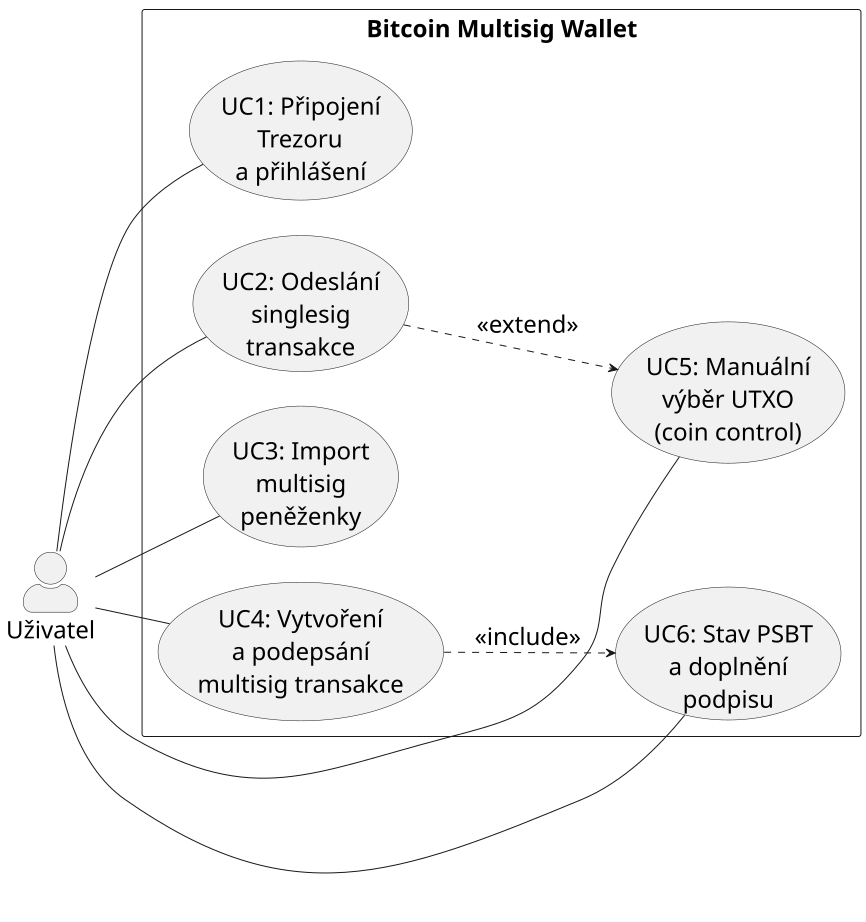
\includegraphics[width=\textwidth]{img/use-case.pdf}
\caption{Diagram případů užití. Uživatel interaguje se~systémem prostřednictvím
osmi hlavních funkcí; coin control rozšiřuje odeslání transakce a~přepnutí účtu
je součástí multisig podepisování.}
\label{fig:use-case}
\end{figure}

%%% -----------------------------------------------------------------------
\section{Funkční požadavky}
\label{sec:funkcni-pozadavky}

Funkční požadavky vycházejí z~výše uvedených user stories a~use cases.
Jsou rozděleny do tří oblastí; u~každého požadavku uvádíme vazbu na
příslušné US/UC.

\subsection{Autentizace a správa účtů}

\begin{description}
  \item[F1 -- Přihlášení přes Trezor \textnormal{(US1, UC1)}:]
    Systém umožní přihlášení prostřednictvím hardwarové peněženky Trezor
    s~využitím deeplink mechanismu (přesměrování do~jiné aplikace
    prostřednictvím speciální URL) Trezor Connect~\cite{TrezorConnect}.
    Při přihlášení aplikace vyžádá z~Trezoru deset rozšířených veřejných
    klíčů (xpub) pro derivační cesty tvaru \texttt{m/84'/c'/N'} dle
    BIP-84~\cite{BIP84}, kde \texttt{N} je v~rozsahu 0 až 9 a~\texttt{c}
    nabývá hodnoty 0 pro mainnet a~1 pro testnet.

  \item[F2 -- Discovery účtů \textnormal{(US1, UC1)}:]
    Backend pro každý přijatý xpub odvodí dávku adres podle BIP-44 gap
    limitu~\cite{BIP44} a~ověří na blockchainu, zda mají transakční
    historii. Pro účty s~nalezenou aktivitou automaticky vytvoří
    peněženky.

  \item[F3 -- Přepínání účtů \textnormal{(US10)}:]
    Systém umožní přepínání mezi singlesig a~multisig peněženkami
    prostřednictvím navigačního menu. Každý singlesig účet je hlavním
    účtem a~může mít přidružené multisig peněženky importované
    prostřednictvím deskriptorů.
\end{description}

\subsection{Singlesig transakce}

\begin{description}
  \item[F4 -- Zobrazení zůstatku \textnormal{(US2)}:]
    Systém zobrazí aktuální zůstatek peněženky v~BTC a~v~přepočtu na fiat
    měnu s~využitím směnného kurzu z~CoinGecko API~\cite{CoinGeckoAPI}.

  \item[F5 -- Odeslání prostředků \textnormal{(US3, UC2)}:]
    Systém umožní odeslání Bitcoinu na zadanou adresu (singlesig P2WPKH).
    Poplatek je vypočten deterministicky na základě počtu vstupů, výstupů
    a~uživatelem zvoleného fee rate (sat/vB).

  \item[F6 -- Příjem prostředků \textnormal{(US4)}:]
    Systém umožní příjem Bitcoinu zobrazením přijímací adresy a~QR kódu.

  \item[F7 -- Historie transakcí \textnormal{(US11)}:]
    Systém zobrazí historii transakcí včetně detailů (částka, adresa,
    poplatek, stav potvrzení).

  \item[F8 -- Coin control \textnormal{(US5, UC5)}:]
    Systém poskytne funkci manuálního výběru konkrétních UTXO jako vstupů
    transakce; poplatek je přepočítán při sestavení PSBT podle počtu
    vybraných vstupů.
\end{description}

\subsection{Multisignature transakce}

\begin{description}
  \item[F9 -- Import multisig peněženky \textnormal{(US6, UC3)}:]
    Systém umožní import multisig peněženky zadáním deskriptoru ve formátu
    \texttt{wsh(sortedmulti(\ldots))} dle BIP-380~\cite{BIP380}
    a~BIP-383~\cite{BIP383}. Deskriptor lze do aplikace dostat textovým
    vložením ze schránky nebo naskenováním QR kódu. Z~deskriptoru systém
    extrahuje práh M, veřejné klíče cosignerů a~derivační cesty dle
    BIP-48~\cite{BIP48}.

  \item[F10 -- Vytvoření PSBT \textnormal{(US7, UC4)}:]
    Systém umožní vytvoření částečně podepsané transakce ve formátu
    PSBT~\cite{BIP174} pro multisig peněženku. Veřejné klíče v~redeem
    skriptu jsou řazeny dle BIP-67~\cite{BIP67} na úrovni odvozených
    klíčů pro každý vstup.

  \item[F11 -- Podepsání PSBT \textnormal{(US7, US9, UC4, UC6)}:]
    Systém umožní podepsání PSBT prostřednictvím Trezoru s~derivační
    cestou odpovídající aktuálnímu cosignerovi.

  \item[F12 -- Stav PSBT \textnormal{(US8, UC6)}:]
    Systém zobrazí stav rozpracovaných PSBT -- počet shromážděných
    podpisů, chybějící cosigneři -- a~umožní doplnění podpisu dalším
    cosignerem.

  \item[F13 -- Broadcast transakce \textnormal{(UC4)}:]
    Po~dosažení prahu podpisů zmizí na~detailu PSBT tlačítko
    \emph{Sign with Trezor} a~místo něj se zobrazí \emph{Broadcast
    Transaction}. Po~jeho stisknutí aplikace zavolá broadcast
    endpoint a~finalizovanou transakci propaguje do~Bitcoin sítě.
    Broadcast je tedy explicitní akcí některého cosignera
    na~detailu PSBT -- po~přijetí posledního podpisu se transakce
    sama od~sebe neodesílá a~iniciuje ji vždy klient, nikoli
    server-side background úloha.
\end{description}

%%% -----------------------------------------------------------------------
\section{Nefunkční požadavky}
\label{sec:nefunkcni-pozadavky}

Nefunkční požadavky specifikují kvalitativní vlastnosti systému.

\subsection{Bezpečnost}

\begin{description}
  \item[NF1 -- Privátní klíče mimo server:]
    Server nikdy nedisponuje privátními klíči uživatele. Veškeré podepisování
    transakcí probíhá výhradně na hardwarové peněžence Trezor. Server pracuje
    pouze s~veřejnými klíči (xpub) a~nepodepsanými nebo částečně podepsanými
    transakcemi (PSBT).

  \item[NF2 -- Autentizace:]
    Komunikace mezi mobilní aplikací a~backendem je autentizována pomocí
    JWT tokenů (JSON Web Token -- digitálně podepsaný přístupový token
    nesoucí identitu zařízení). Token je vydán při přihlášení a~vázán
    na~deterministicky odvozený \texttt{deviceId} z~kořenového otisku
    Trezoru, takže opakovaná přihlášení ze~stejného zařízení vedou
    na~stejnou identitu.

  \item[NF3 -- Důvěryhodný síťový kanál:]
    Komunikace mezi aplikací a~backendem probíhá přes HTTP v~izolované
    LAN nebo ve~VPN (ve~vývojovém nasazení používáme Tailscale, které
    zajišťuje šifrování na~síťové vrstvě mezi zařízeními). TLS
    na~aplikační vrstvě není v~rámci této práce řešeno.
\end{description}

\subsection{Platforma a kompatibilita}

\begin{description}
  \item[NF4 -- Cílová platforma:]
    Mobilní aplikace je určena pro platformu Android s~minimální podporovanou
    verzí API~24 (Android~7.0) a~cílovou verzí API~34 (Android~14).

  \item[NF5 -- Hardwarová peněženka:]
    Systém vyžaduje hardwarovou peněženku Trezor řady Safe (modely Safe~3,
    Safe~5 nebo Safe~7; starší Trezor One není podporován) a~nainstalovanou
    aplikaci Trezor Suite Mobile, která slouží jako prostředník pro
    podepisování transakcí (podrobnou analýzu tohoto rozhodnutí
    a~zvažovaných alternativ uvádíme v~sekci~\ref{sec:analyza-trezor}).
    Peněženka se k~mobilnímu zařízení připojuje USB-C kabelem
    (Safe~3, Safe~5) nebo bezdrátově přes Bluetooth (pouze Safe~7).
\end{description}

\subsection{Použitelnost}

\begin{description}
  \item[NF6 -- Asynchronní operace:]
    Síťové operace (načítání zůstatku, broadcast transakce) probíhají asynchronně
    a~neblokují uživatelské rozhraní. Uživatel je o~probíhající operaci informován
    vizuálním indikátorem.
\end{description}

\subsection{Testovatelnost}

\begin{description}
  \item[NF7 -- Podpora testnetu:]
    Systém podporuje Bitcoin testnet4 (nejnovější testovací síť Bitcoinu,
    nástupce testnet3) pro účely vývoje a~testování bez rizika ztráty
    reálných prostředků. Trezor používá pro testnet stejné derivační cesty
    (\texttt{coin\_type = 1}) nezávisle na verzi testnetové sítě -- volba
    testnet4 se týká blockchainového API (Mempool.space). Přepínání
    mezi testnetem a~mainnetem provádí uživatel na přihlašovací obrazovce
    mobilní aplikace.
\end{description}
